\section{Производственная и экологическая безопасность}
\subsection{Обеспечение безопасных условий труда при разработке и испытании информационной системы}

Целью дипломного проекта является создание ПС определения вероятных мест скопления людей в помещениях,
направленного на решение актуальных задач, возникающих при разработке архитектурных проектов.
Разрабатываемое ПС позволяет решать задачи обеспечения безопасности, оптимизации путей эвакуации,
максимизации прибыли путем определения наиболее привлекательных мест установки коммерческих объектов и многие другие.
При разработке ПС определения вероятных мест скопления людей в помещениях был проведен анализ аналогов на современном рынке,
в результате которого был выработан набор требований, позволяющий соединить в себе все преимущества аналогов и избежать их недостатков.
В соответствии с предъявленными требованиями для разработки ПС были выбраны наиболее подходящие языки программирования и модели, такие как
языки программирования Ruby, Rust и C; модель социальных сил в качестве модели пешеходных потоков.

В настоящем разделе рассмотрим вопросы, связанные с обеспечением безопасности при разработке и испытании информационной системы.

Основным инструментом разработчика информационной системы является персональный компьютер.
При разработке данного дипломного проекта с использованием персонального компьютера решались следующие задачи:
  кодирование и тестирование ПС "--- с помощью текстового редактора Vim версии 7.4, эмулятора терминала urxvt версии 9.21, а так же компиляторов и интерпретаторов используемых языков программирования Ruby (версия 2.2), Rust (версия 1.0) и C (компилятор gcc версии 4.9.2);
  оформление сопроводительных документов "--- с помощью системы компьютерной верстки TeX версии 3.14159265 (реализована проектом livetex версии 2014.36709), а также набора макрорасширений LaTeX версии 2e.
Используемый персональный компьютер обладает следующей конфигурацией: процессор "--- Intel Core i3-4130, оперативная память "--- Kingston DDR3 8 Gb,
  система охлаждения процессора "--- Zalman CNPS10X Optima, твердотельный накопитель (хранилище данных) "--- SPCC Solid State Disk 120GB,
  монитор "--- Samsung SyncMaster BX2231.
Данный персональным компьютер изображен на рисунке~\ref{ot_pc_pic}.

\begin{figure}[ht!]
  \begin{center}
    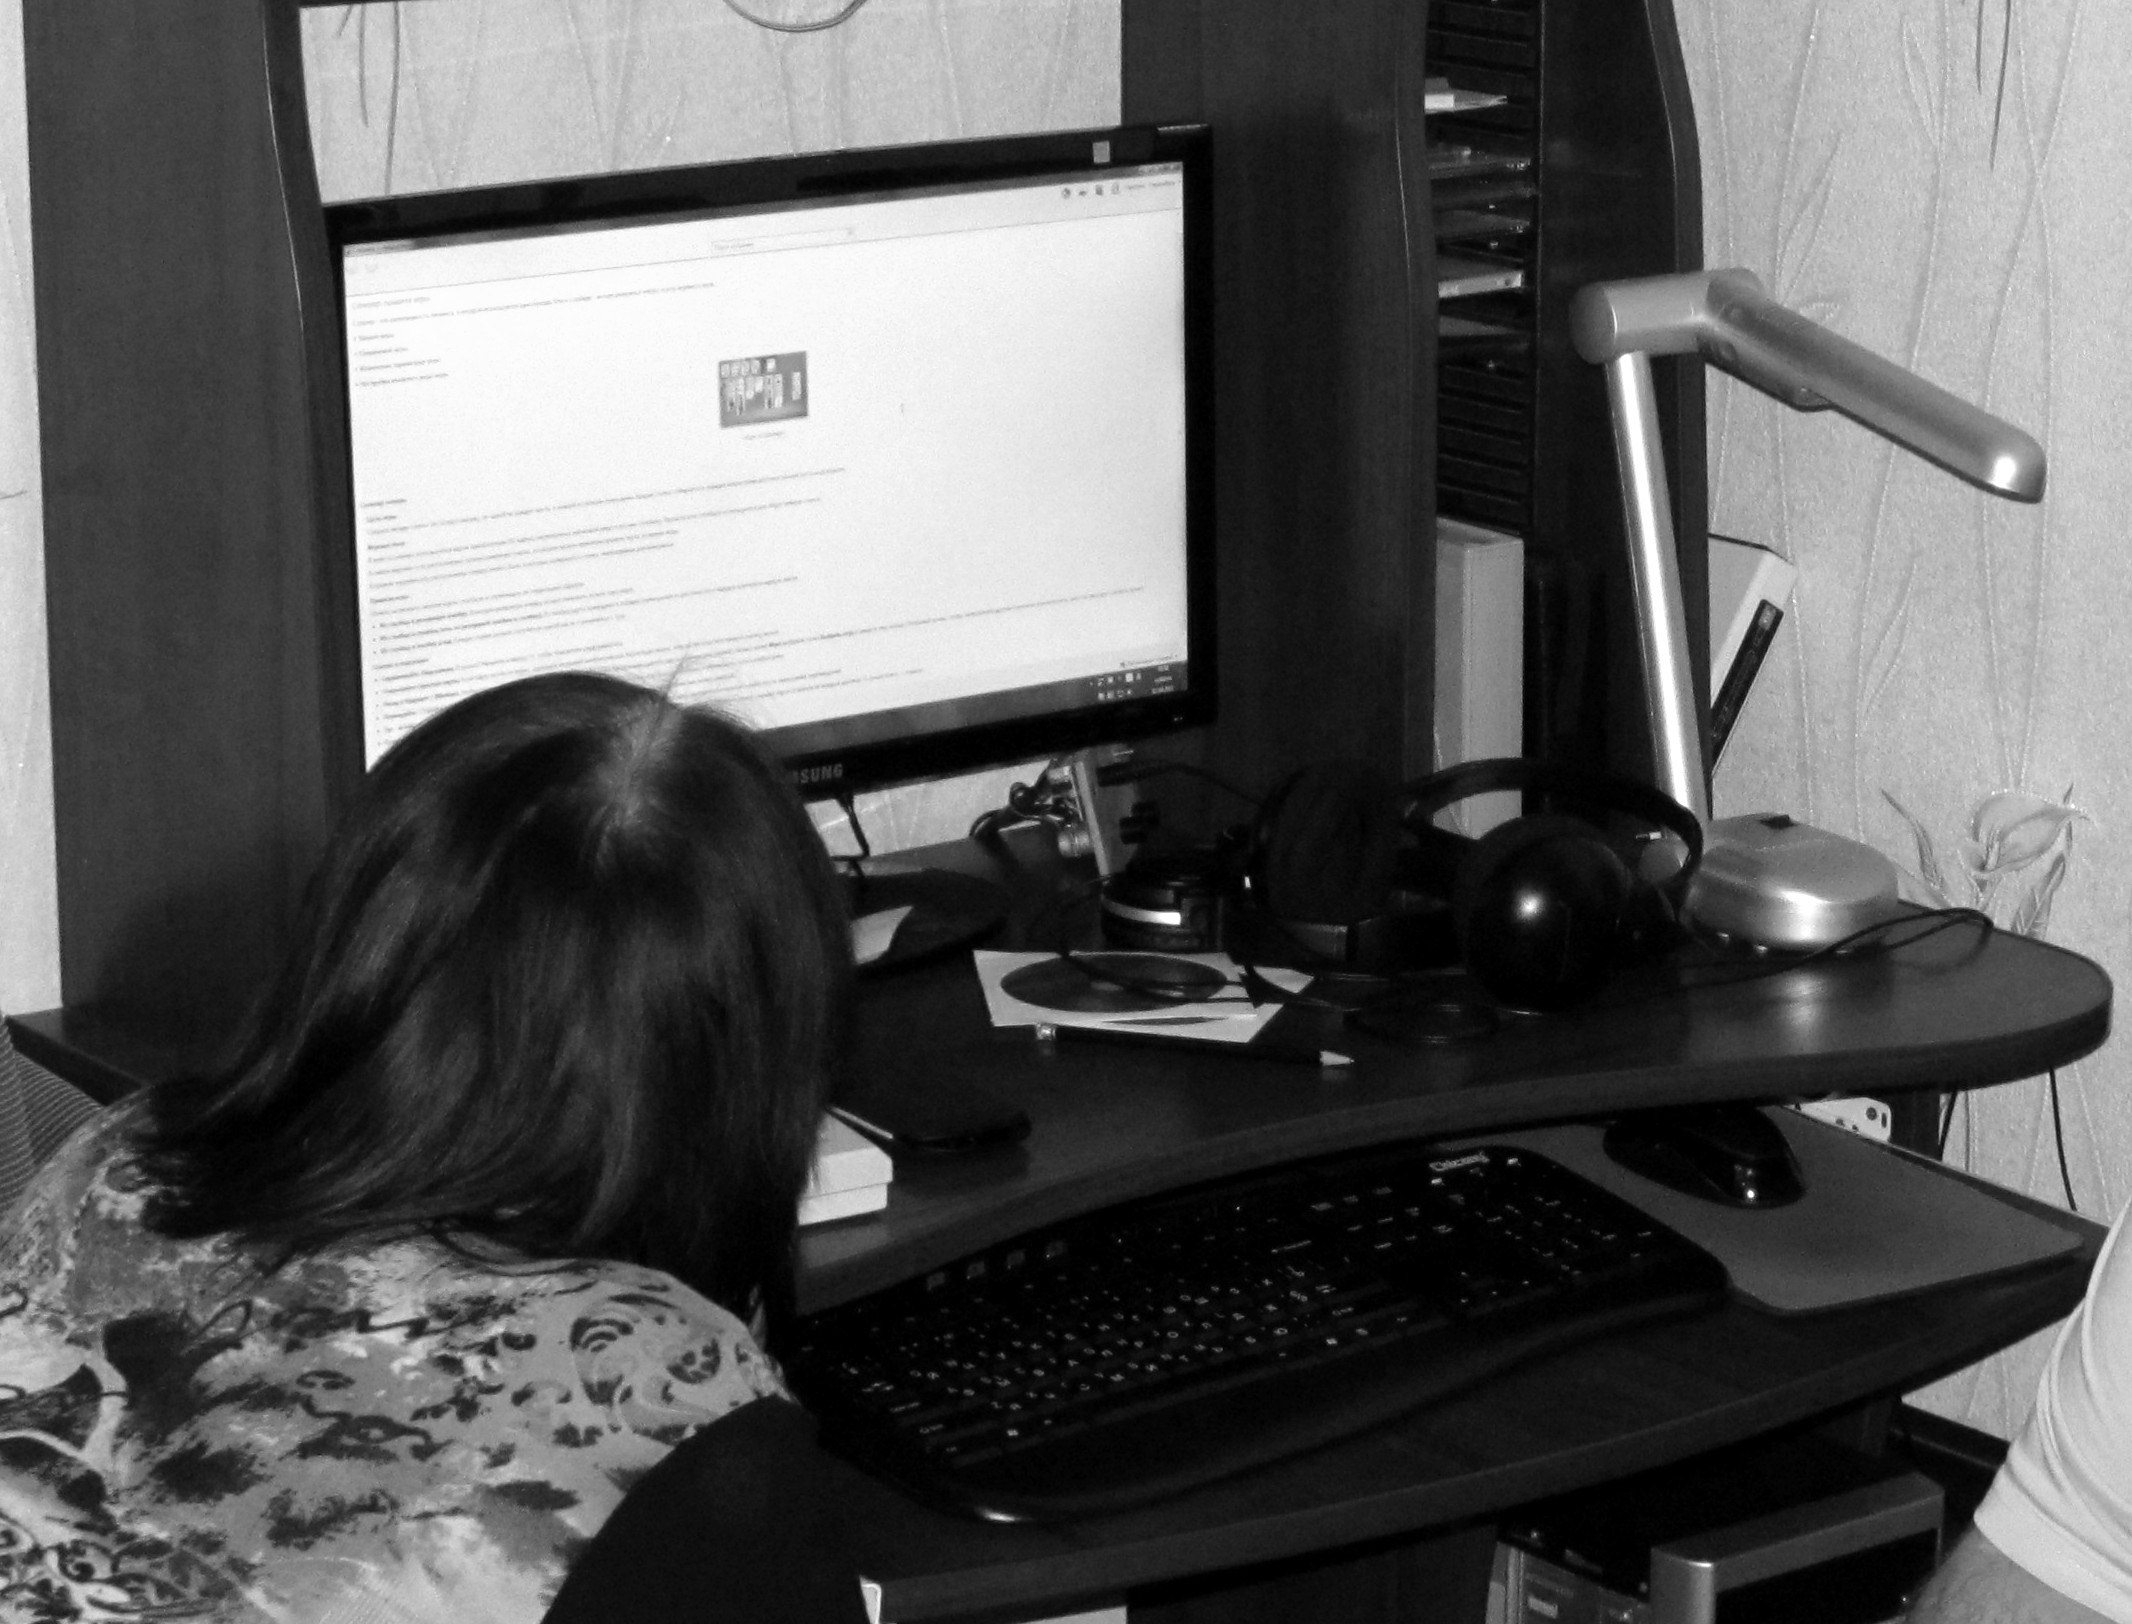
\includegraphics[width=250px]{comp}
    \caption{Используемый при разработке персональный компьютер}
    \label{ot_pc_pic}
  \end{center}
\end{figure}

Персональный компьютер является источником ряда опасных факторов, способных нанести вред здоровью разработчика.
К таким факторам относят электромагнитное излучение, ионизирующее излучение, шум, вибрации и другие.
Также при работе на персональном компьютере возникает ряд опасных факторов, источником которых не является сам персональный компьютер.
Например, такими факторами могут являться повышенная зрительная нагрузка, длительное неизменное положение тела в пространстве и другие.
В оставшейся части данного раздела будут более подробно рассмотрены названные выше опасные факторы
и будут предложены способы минимизации вреда от данных факторов при разработке ПС.

Первым названным фактором является электромагнитное излучение.
ПК является источником электромагнитного излучения с широким диапазоном частот от 5 Гц до 800 МГц~\cite{ot_emr_pc}.
Одним из основных источников электромагнитного излучения в персональном компьютере является монитор.
В качестве технических стандартов безопасности дисплеев персональных компьютеров используются
  международный стандарт ISO 9241;
  шведские стандарты MPR II, ТСО'91/92/95/99/03;
  американский стандарт FCC;
  российские стандарты ГОСТ Р 50948"=96, ГОСТ Р 50949"=96, СанПиН 2.2.2.542"=96~\cite{ot_emr_pc}.
На территории Республики Беларусь действует стандарт СанПиН 9"=131 РБ 2000 <<Гигиенические требования к видеодисплейным терминалам, электронно"=вычислительным машинам и организации работы>>.
В частности в этом документе описаны предельно допустимые уровни электромагнитного излучения для мониторов.
Для минимизации вредного воздействия электромагнитного излучения в ходе разработки ПС было принято решение оборудовать рабочие места программистов только сертифицированными компонентами персональных компьютеров. При этом особое внимание уделить наличию сертификата у монитора, а так же проверить его уровни излучения на соответствие международным стандартам.

Следующим фактором является ионизирующее излучение.
Основным источником ионизирующего излучения в персональном компьютере является монитор, основанный на технологии электронно"=лучевой трубки.
Данный тип мониторов считается устаревшим, и при разработке ПС было решено использовать мониторы технологии жидких кристаллов,
что позволяет свести на нет влияние ионизирующего излучения при работе за персональным компьютером.

Также важными факторами при работе за персональным компьютером являются шум и вибрация.
Шум и вибрация возникают из"=за движения механических частей.
Их рассмотрение производится вместе по причине того, что в персональном компьютере основные источники шума и вибрации совпадают "--- это охлаждающая система и жесткий диск.
Наиболее распространенной охлаждающей системой является система на основе радиаторов и кулеров (вентиляторов).
При этом источником шума и вибрации, очевидно, являются именно кулеры.
Существуют и другие системы охлаждения на основе жидкости, однако чаще всего их применение неоправданно дорого.
С целью минимизации шума и вибраций от охлаждающей системы были приняты несколько решений.
Первое решение "--- использовать процессоры фирмы Intel. Эти процессоры обладают гораздо меньшей тепловой мощностью по сравнению с их основным конкурентом "--- фирмой AMD.
Это позволит поставить систему охлаждения, рассчитанную на меньший теплоотвод, а следовательно и производящую меньший уровень шума и вибраций.
Второе решение "--- выделить несколько больший бюджет на приобретение охлаждающей системы. Это позволит приобрести более дорогую модель с меньшим уровнем шума и вибраций.
Также источником шума и вибрации является жесткий диск.
К счастью, не так давно появилась немеханическая альтернатива жестким дискам "--- твердотельные накопители.
Замена жесткого диска на твердотельный накопитель позволяет полностью избавиться от шума и вибраций, а так же получить более высокую производительность.
Платой за данные преимущества является цена и надежность, однако на современном этапе можно выбрать твердотельный накопитель с приемлемой ценой и надежностью.
Также можно перенести хранение программного кода с персонального компьютера разработчика на облачный сервер, что уменьшит последствия потери информации.
В связи с этим было решено использовать твердотельный накопитель в качестве хранилища данных на персональных компьютерах разработчиков.

Рассмотрим еще один фактор, влияющий на безопасность работы за персональным компьютером "--- повышенная зрительная нагрузка.
При работе за персональным компьютером наибольшую физиологическую нагрузку получают глаза.
Это связано с тем, что монитор персонального компьютера в силу технических ограничений не может достаточно точно воспроизвести реальность.
Существует четыре основных особенности изображения на экране монитора.
Первая особенность "--- изображение на экране монитора является плоским. Это заставляет систему аккомодации глаза находиться в одном статическом состоянии, в то время как в реальности фокус зрения постоянно меняется. Это приводит к развитию различных нарушений аккомодации.
Вторая особенность "--- изображение на экране монитора само является источником света, а не отражает свет. Зрительная система человека плохо адаптирована к длительному рассмотрению светящихся объектов~\cite{ot_long_work_pc}. Также спектр излученного монитором света значительно отличается от спектра естественного света, что тоже влияет на удобство восприятия изображения.
Третья особенность "--- низкий контраст изображения. Контрасту мониторов всегда уделялось особое внимание, и современные мониторы имеют достаточно неплохой показатель контрастности. Однако до идеального значения ему все же далеко.
Четвертая особенность "--- наличие мерцания изображения. На современных жидкокристаллических мониторах данную проблему удалось почти полностью устранить.
Степень влияния этих особенностей напрямую зависит от качества монитора. Именно поэтому для разработчиков ПС должны быть приобретены качественные мониторы.
Также для уменьшения влияния статического фокуса рекомендуется делать перерывы в работе за монитором.
Общей рекомендацией является делать перерывы на 10"=15 минут каждые 1,5"=2 часа работы.
Во время перерывов желательно делать упражнения для глаз.

Последним рассматриваемым фактором является длительное неизменное положение тела в пространстве.
При вынужденной длительной неизменной рабочей позе возникает статическая нагрузка на мышцы ног, плеч, шеи и рук, которые длительно пребывают в состоянии сокращения.
Поскольку мышцы не расслабляются, в них ухудшается кровоснабжение; нарушается обмен веществ, накапливаются биопродукты распада.
Это приводит к мышечной слабости и другим мышечным расстройствам.
Также увеличивается нагрузка на опорный аппарат, в частности на позвоночник. Это может привести к изменению его формы, что является причиной множества побочных заболеваний~\cite{ot_back_diseases}.
Избавиться от влияния данного фактора невозможно.
Единственной рекомендацией является делать перерывы во время работы, однако даже регулярные перерывы не способны полностью устранить влияние этого фактора.

Таким образом, изложенные выше предложения обеспечивают безопасность при разработке и испытании информационной системы.
